\subsection{Introduction to Time Series}
Models are not always \textit{independent of the order} of the training data. Many real life measuring and data recording processes result in data sets that are \textit{serially correlated}. For example \textit{machine monitoring, stock, environmental observations or federal statistics.} These kind of data is called \textit{time series data}. Usually there are several goals that one wants to achieve in time series data.
\begin{itemize}
	\item \textbf{Descriptive Analysis}
	\item \textbf{Modelling and Interpretation}
	\item \textbf{Decomposition}
	\item \textbf{Predection}
	\item \textbf{Regression}
\end{itemize}
\todo{Chapter 13}
\subsubsection{Time Series with \color{blue}R}
{
\RTheory
{	All data in {\color{blue}R} are stored in objects, which provide a range of methods. The class of an object can be found using the {\color{blue}class} function. For example, we have already encountered the {\color{blue}data.frame} class. It has a series of methods, such as {\color{blue}names} or {\color{blue}nrow}: \vfill
(The data set iris contains 50 samples of three types of Iris flowers, measured along four variables.)}
{sections/TimeSeriesAnalysis/IntroductionToTimeSeries/RCode/timeSeries.R}
\paragraph{The {\color{blue}ts} Class}
{\RTheory
{\textbf{Basic properties:}\vfill
	The AirPassengers-data is a built in set of class {\color{blue}ts}. Most important methods for {\color{blue}ts} class are:\vfill 
\begin{enumerate}
\item  {\color{blue}start()} returns the start time of the series.
\item  {\color{blue}end()} returns the end time of the series.
\item  {\color{blue}frequency()} returns the number of samples per unit time.
\item  {\color{blue}plot()} displays the time series as a function over the time axis. {\color{blue}plot} function calls {\color{blue}plot.ts} which is tailored for time series. See Figure AirPassengers. 
\end{enumerate}}
{sections/TimeSeriesAnalysis/IntroductionToTimeSeries/RCode/tsClassBasic.R}
\begin{figure}[H]\centering
	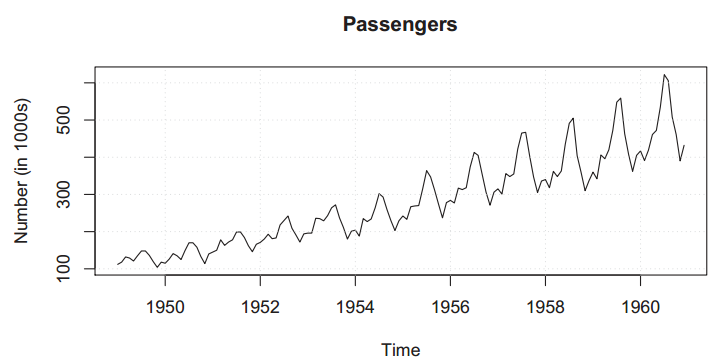
\includegraphics[width=0.7\linewidth]{images/tsAirPassengers.png}
	\caption{AirPassengers}
	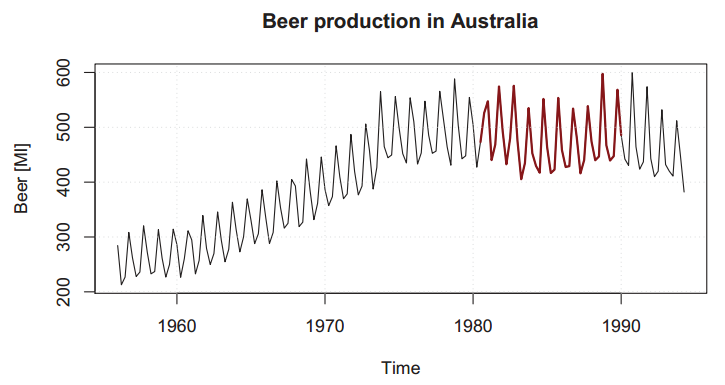
\includegraphics[width=0.7\linewidth]{images/tsSeasBehav.png}
	\caption{Subset of a Time Series (seasonal behaviour)}
\end{figure}
\RTheory
{
\textbf{Defining a {\color{blue}ts} class}\vfill
If data is not in a time series form we can make a {\color{blue}ts} object by using the {\color{blue}ts}  function. This is not necessary for AirPassengers, therefore the example AustralianBeer is used.
\begin{enumerate}
	\item  {\color{blue}summary()} gives the five-number summary as well as the mean of the time series.This function shows the minimum, the first quartile, the median, the second quartile and the maximum of the time series. This is called the \textit{five-number-summary} of a data set. Additionally the mean is also computed.
	\item  {\color{blue}window()} returns a subset of the time series defined by a start and an end time.
\end{enumerate}
}
{sections/TimeSeriesAnalysis/IntroductionToTimeSeries/RCode/tsClassDefining.R}

}



}